\documentclass[tikz,border=8pt]{standalone}
\begin{document}
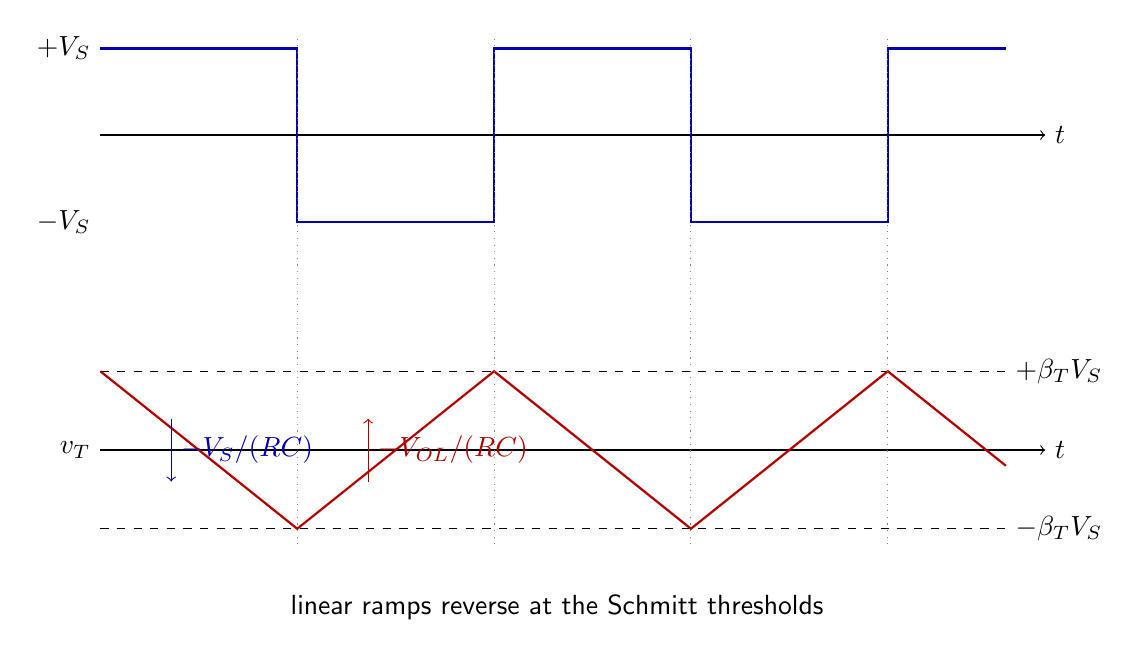
\begin{tikzpicture}[font=\sffamily,x=1cm,y=1cm]
\draw[->] (0,0)--(12,0) node[right]{$t$};
\draw[blue!70!black,thick] (0,1.1)--(2.5,1.1)--(2.5,-1.1)--(5,-1.1)--(5,1.1)--(7.5,1.1)--(7.5,-1.1)--(10,-1.1)--(10,1.1)--(11.5,1.1);
\node[left] at (0,1.1) {$+V_S$}; \node[left] at (0,-1.1) {$-V_S$};
\draw[->] (0,-4)--(12,-4) node[right]{$t$};
\draw[dashed] (0,-3)--(11.5,-3) node[right]{$+\beta_T V_S$};
\draw[dashed] (0,-5)--(11.5,-5) node[right]{$-\beta_T V_S$};
\draw[red!70!black,thick] (0,-3)--(2.5,-5)--(5,-3)--(7.5,-5)--(10,-3)--(11.5,-4.2);
\foreach \x in {2.5,5,7.5,10}{\draw[gray,dotted] (\x,-5.2)--(\x,1.25);}
\node[left] at (0,-4) {$v_T$};
\draw[->,blue!70!black] (.9,-3.6)--(.9,-4.4) node[midway,right]{$-V_S/(RC)$};
\draw[->,red!70!black] (3.4,-4.4)--(3.4,-3.6) node[midway,right]{$-V_{OL}/(RC)$};
\node at (5.8,-6) {linear ramps reverse at the Schmitt thresholds};
\end{tikzpicture}
\end{document}
